\documentclass{paper}
\usepackage[colorlinks=true, linkcolor=blue, citecolor=blue, urlcolor=magenta]{hyperref}
\usepackage{float}
\usepackage{array}
\usepackage{ragged2e}
\usepackage{graphicx}



% Title Information
\title{Early Parkinson's Detection Through Speech Analysis}
\author{Manuel Cortez Muñoz\textsuperscript{1}}
\affiliation{School of Engineering, Universidad Autónoma de San Luis Potosí,
San Luis Potosí, México}
\email{\texttt{manuelcortezm}@outlook.com}

% Document Start
\begin{document}

\maketitle
\thispagestyle{firstpage}
% Abstract Section
\begin{abstract}
Parkinson's disease (PD) often affects the voice before diagnosis, which makes speech a candidate for low-cost screening. This study evaluates machine learning models that classify PD from 81 sustained vowel recordings captured over the telephone at 8 kHz (41 healthy controls, 40 participants with PD). A first version of this work reported 82.72\% accuracy for an SVM on five MFCC features. That estimate relied on feature selection and threshold tuning that used the test data, and on a CNN early-stopped on its own test fold. Under repeated stratified 5-fold cross-validation with every choice made inside the training folds, the SVM reaches 71.6\% accuracy (AUC 0.78) and the CNN 60.0\% (AUC 0.67). The two groups also differ by 19 years in mean age: a model given only age and sex reaches 81.8\% accuracy (AUC 0.86), and adding voice features to it does not improve performance. In an age-matched subgroup, a weak voice signal remains (AUC 0.66, permutation $p = 0.037$, 11 controls). On this dataset, voice-based detection of PD cannot be separated from age, and larger age-matched cohorts are needed before clinical use.
\\
\\
\textbf{Keywords:}
Parkinson's disease, Speech analysis, Machine learning, Cross-validation, Selection bias, Confounding
\end{abstract}

% Sections
\section{Introduction}
Parkinson’s disease (PD) is a neurodegenerative disorder that affects the nervous system. It was first described as a neurological condition in 1817~\cite{bloem2021parkinson}. It is one of the most common neurodegenerative disorders in the world, with an incidence rate of approximately 20/100,000 and a prevalence rate exceeding 100/100,000~\cite{rajput2007epidemiology, von2005prevalence}. PD  impacts motor functions, with symptoms such as bradykinesia, rigidity, rest tremor, and postural instability~\cite{postuma2015mds, virameteekul2023clinical}. 
PD is a complex disease, and its clinical diagnosis is not always straightforward. Traditionally, diagnosis has been based on clinical features and subjective rating scales, which have made early and accurate detection challenging~\cite{schrag2002valid}.

PD is caused by the progressive degeneration of neurons in a specific part of the brain called the substantia nigra. The substantia nigra is responsible for producing dopamine, a neurotransmitter that helps control movement. As these neurons are damaged, dopamine production decreases, leading to the motor symptoms commonly associated with PD. The reduction in dopamine disrupts communication between the brain regions that coordinate movement, resulting in the characteristic tremors, rigidity, and slowness of movement seen in patients~\cite{ahmed2022classification}. Speech abnormalities are also a common early sign of the disease, about 89\% of individuals with PD experience speech disorders like uncertain articulation, hoarse and breathy voice, and monotone pitch ~\cite{ahmed2022classification}. These changes are also a consequence of the degeneration of the substantia nigra and the resulting dopamine deficiency.

This project aims to use techniques and algorithms such as Machine Learning, Transfer Learning, Deep Learning to investigate different features of raw audio files. These are for the early detection of PD through speech analysis of audio files. My motivation for this research stems from the fact that PD is an incurable disease and the degeneration it causes is debilitating. Detecting early PD is crucial for a better management of symptoms, but current diagnostic methods remain complex and difficult to access. By exploring the potential of studying features from audio signals as a diagnostic complement. This research seeks to identify features and test models that could enable a binary classification system, determining whether a person may have PD based on their speech patterns.

Given the profound impact of neurological disorders like PD on the lives of patients and their families, it is essential to explore new methods of early diagnosis. 

More than one million people in North America alone are affected by PD, and while medication exists to alleviate symptoms, especially in the early stages, there is currently no cure~\cite{ae1998parkinson, singh2007advances}. The development of machine learning-based decision support tools that can differentiate between healthy individuals and people with PD could provide a promising solution to this challenge~\cite{little2008suitability, sapir2010formant}.


% Subsections
\section{Background and Related Work}
\subsection{Parkinson’s Disease and Speech Disorders}

Parkinson’s disease (PD) is a neurodegenerative disorder that not only affects motor functions but also has a profound impact on speech. Research has shown that approximately 90\% of people with Parkinson’s (PWP) exhibit some form of vocal impairment~\cite{ho1999speech, logemann1978frequency}. This vocal impairment may be one of the earliest indicators of the disease, often detectable up to five years before a clinical diagnosis is confirmed~\cite{duffy2012motor}. Due to the noninvasive and easily administered nature of voice measurement, speech analysis has gained significant attention as a potential tool for detecting and monitoring PD progression~\cite{sapir2007effects, rahn2007phonatory}.

The range of speech symptoms associated with PD includes reduced loudness, increased vocal tremor, and breathiness (noise)~\cite{tsanas2012novel}. These changes are primarily due to the degeneration of the nervous system, which affects the muscles responsible for speech production. The vocal impairments seen in PD can be categorized into two major disorders:

\begin{itemize}
    \item \textbf{Dysphonia}: A condition characterized by the inability to produce normal vocal sounds, leading to hoarseness, weak voice, and breathy speech.
    \item \textbf{Dysarthria}: A motor speech disorder that affects the articulation of words, making speech slurred and less intelligible.
\end{itemize}

These speech abnormalities result from the loss of fine motor control in the vocal muscles, which is directly linked to dopamine depletion in the substantia nigra. Given that speech disorders are present in most individuals with PD and can serve as early indicators of the disease, machine learning techniques applied to speech analysis offer a promising approach for identifying PD at an early stage. A more detailed description of speech disorders can be found in~\cite{baken1987clinical}.

\subsection{Speech as a Diagnostic Tool for Parkinson’s Disease}

The clinical diagnosis of Parkinson’s disease (PD) is highly dependent on expert evaluation. When strict clinical diagnostic criteria are applied by specialists, the accuracy of diagnosis can reach over 97\% over a patient’s lifetime and 91.5\% within the first five years of the disease~\cite{virameteekul2023clinical}. However, for non-experts, diagnostic accuracy is significantly lower, at 77\% over a lifetime and 76\% in the first five years~\cite{virameteekul2023clinical}. Furthermore, even for trained professionals, achieving high confidence in a diagnosis takes time. As a result, many individuals with PD go years without an official diagnosis until their symptoms become more pronounced and easily recognizable. While rest tremor is one of the most commonly associated symptoms, it does not manifest in all patients. Additionally, many people may attribute early signs of PD, such as gait changes, balance issues, and cognitive decline, to normal aging, further delaying diagnosis.

Speech-related symptoms, however, provide an early and easily measurable indication of PD. One of the first noticeable speech symptoms in PD is \textbf{hypophonia}—a condition characterized by low-amplitude speech~\cite{ho1999speech}. While hypophonia is the most recognizable speech-related feature in clinical settings, other speech abnormalities commonly observed in PWP include:

\begin{itemize}
    \item \textbf{Hoarseness}: A rough, breathy vocal quality.
    \item \textbf{Dysarthria}: Slurred or imprecise articulation of words.
    \item \textbf{Tachyphemia}: Rapid, stuttering speech that can make communication difficult~\cite{logemann1978frequency, vercruysse2012freezing}.
\end{itemize}

Speech is a complex cognitive-motor skill that relies on precise coordination between the vocal motor system and the cognitive networks responsible for language production and comprehension. These systems are highly susceptible to neurodegenerative changes in PD, leading to the observed speech impairments~\cite{smith2018communication, rusz2013imprecise}. 

The potential of voice measurements as objective metrics for detecting and tracking PD progression has been widely studied, with most research conducted in controlled laboratory environments. However, a promising avenue of research lies in the development of automated tools capable of detecting speech changes even before the onset of overt motor symptoms, potentially aiding in earlier diagnosis~\cite{postuma2016voice}.

Early diagnosis is crucial for the development of neuroprotective strategies, as it is estimated that by the time PD is clinically diagnosed, approximately 50\% of the dopaminergic neurons in the substantia nigra pars compacta have already degenerated~\cite{blesa2022motor, schapira2017non}. Furthermore, since voice recording is \textit{non-invasive}, \textit{easy to administer}, and can be performed both in clinical settings and remotely~\cite{virmani2022feasibility}, speech analysis could also serve as an effective method for tracking disease progression over time~\cite{skodda2009progression}.

\subsection{Machine Learning for Parkinson’s Detection}

Machine learning has been extensively applied to the classification of Parkinson’s disease (PD) using voice features. Various algorithms, including Random Forest (RF), Support Vector Machines (SVM), Convolutional Neural Networks (CNN), and Recurrent Neural Networks (RNN), have been explored for detecting PD through speech analysis. The primary goal is to extract relevant acoustic features from voice recordings and leverage them to differentiate individuals with PD from healthy controls.

Among traditional machine learning approaches, RF and SVM have been widely used for PD classification. RF, an ensemble learning technique that combines multiple decision trees, has demonstrated robustness to parameter tuning and high classification accuracy~\cite{hastie2009elements,breiman2001random}. Conversely, SVMs seek to find an optimal hyperplane that separates individuals with PD from healthy subjects. When the data is not linearly separable, SVMs utilize kernel functions to transform the feature space, thereby enhancing classification performance~\cite{hastie2009elements}.

Recent studies have also investigated the effectiveness of machine learning models in real-world conditions.~\citet{carron2021mobile} analyzed the impact of uncontrolled and unsupervised voice recordings on PD classification performance. Their study compared high-quality voice recordings obtained in laboratory settings with smartphone-based recordings from the mPower database~\cite{bot2016mpower}. The results indicated that while the Passive Aggressive classifier achieved high accuracy (AUC: 0.8–0.9) with controlled recordings, its performance dropped (AUC: 0.6–0.7) when using smartphone-based recordings. This suggests that while smartphone-based voice analysis is a promising approach, its reliability in clinical settings remains uncertain. Another study demonstrated a strong correlation between voice parameters recorded with smartphones and professional microphones, highlighting the potential for reliable PD detection in controlled environments~\cite{uloza2015exploring}.

Although traditional machine learning models like RF and SVM have demonstrated strong performance, deep learning approaches (e.g., CNNs and RNNs) are gaining traction in PD voice analysis. These models can capture more complex patterns in speech data, potentially improving early detection accuracy. However, challenges remain, particularly regarding data quality, feature extraction standardization, and real-world deployment.

Table~\ref{tab:ml_pd}, based on the work of \citet{bind2015survey}, summarizes various studies on PD detection using machine learning. It includes details on the models used, dataset descriptions, and reported accuracy rates.

\begin{table}[H]
    \centering
    \caption{Summary of Machine Learning Approaches for PD Detection}
    \label{tab:ml_pd}
    \resizebox{\textwidth}{!}{
        \begin{tabular}{l|l|r|l}
            \hline
            \textbf{Study} & \textbf{Model} & \textbf{Accuracy} & \textbf{Data Description} \\
            \hline
            \citet{guo2010advances} & Neural Network & 92.9\% & Speech dataset \\
            \citet{sakar2010telediagnosis} & SVM & 92.8\% & Speech signal dataset \\
            \citet{little2008suitability} & SVM & 91.4\% & Speech signal dataset \\
            \citet{wroge2018parkinson} & ANN & 86\% & Voice recordings \\
            \citet{ahmed2022classification} & Random Forest & 97.10\% & Voice dataset \\
            \citet{ahmed2022classification} & K-Nearest Neighbors (KNN) & 95.45\% & Voice dataset \\
            \citet{rustempasic2013diagnosis} & Fuzzy C-means & 68.04\% & Speech signal dataset \\
            \citet{rustempasic2013diagnosis} & ANN & 92\% & Speech signal dataset \\
            \citet{khemphila2012parkinsons} & ANN & 82.05\% & Speech signal dataset \\
            \citet{shahbakhi2014speech} & SVM & 94.27\% & Speech signal dataset \\
            \citet{bocklet2011detection} & SVM & 79\% & Speech dataset \\
            \citet{das2010comparison} & NN classifier & 92.9\% & Speech signal dataset \\
            \citet{can2013diagnosis} & PNN & 92.9\% & Voice recordings \\
            \citet{ccauglar2010automatic} & ANN & 96.77\% & PD dataset \\
            \citet{kapoor2011parkinson} & Vector Quantization & 95\% & Audio input \\
            \citet{wu2011data} & Decision Tree and Neural Network & 95\% & Recorded speech signals \\
            \citet{chen2013efficient} & FKNN & 96.07\% & PD dataset \\
            \citet{yadav2012predication} & SVM & 76\% & Recorded speech signals \\
            \citet{azad2013design} & Decision tree & 85.98\% & Voice recordings \\
            \citet{bouchikhi2013parkinson} & SVM & 96.88\% & Voice recordings \\
            \citet{ma2014efficient} & SVM & 99.49\% & Recorded speech signals \\
            \citet{hazan2012early} & SVM & 99.39\% & Speech data \\
            \citet{sriram2013intelligent} & Random Forest & 90\% & Voice dataset \\
            \citet{prashanth2014parkinson} & SVM \& Classification Tree & 89.26\% & De-novo PD dataset \\
            \citet{kaya2011effect} & Entropy-based Discretization & 94.87\% & Audio input \\
            \citet{nivedita2013artificial} & ANN & 96.42\% & Voice recordings \\
            \citet{gharehchopogh2013case} & MLP & 93.22\% & Audio input \\
            \citet{wu2010prediction} & RBFNN & 89.91\% & Data recorded \\
            \citet{luukka2011feature} & Fuzzy entropy & 84.52\% & Voice recordings \\
            \hline
        \end{tabular}
    }
\end{table}

\section{Challenges and Limitations}
Traditional speech analysis methods focus on fundamental frequency (F0), absolute sound pressure level, jitter, shimmer, and noise-to-harmonics ratio (NHR). Studies have shown that individuals with PD exhibit significant variations in these acoustic features compared to healthy individuals, suggesting their usefulness in assessing dysphonia severity~\cite{baken1987clinical, zwirner1991phonatory}. Additionally, research has demonstrated that simple vocal tasks, such as sustaining the vowel sound “ahh…,” can be sufficient for detecting PD and monitoring symptom severity~\cite{little2008suitability, titze2000, tsanas2009accurate, tsanas2011nonlinear}.

These features play a crucial role in the development of machine learning models for PD detection, as they allow algorithms to capture key differences in voice characteristics between individuals with and without PD. Proper selection and preprocessing of these features are essential for improving classification performance and ensuring the robustness of PD detection systems.
Despite the promising results of machine learning models for Parkinson’s disease (PD) detection through voice analysis, several challenges and limitations remain. One of the primary issues is data variability, as voice characteristics can be influenced by numerous factors beyond PD, such as age, gender, language, and even environmental conditions during recording. This variability can introduce noise into the dataset, making it more difficult for models to generalize effectively across diverse populations.

Another major challenge is dataset size and quality. Many studies rely on relatively small datasets, often collected under controlled laboratory conditions, which may not reflect real-world scenarios. As \citet{carron2021mobile} demonstrated, models trained on high-quality, controlled recordings tend to perform better than those using smartphone-based data, highlighting the need for standardized data collection methods.

Audio quality and recording conditions also present significant obstacles. Variations in microphone quality, background noise, and recording devices can impact feature extraction and model performance. While some studies suggest that smartphone recordings can provide reliable diagnostic indicators~\cite{uloza2015exploring}, others indicate that uncontrolled environments can reduce classification accuracy, raising concerns about the clinical reliability of telehealth-based assessments.

Additionally, feature selection and model interpretability remain challenges. While traditional acoustic features such as MFCCs, jitter, and shimmer have shown promise, there is no universal consensus on the most relevant features for PD detection. Moreover, deep learning approaches like CNNs and RNNs, while powerful, often function as "black boxes," making it difficult to understand which speech characteristics contribute most to predictions.

Finally, real-world deployment and clinical validation require further research. Although machine learning models have shown high accuracy in experimental settings, their integration into clinical practice depends on regulatory approval, acceptance by medical professionals, and ease of use for both clinicians and patients. Ensuring that these models perform reliably across different demographics and conditions is crucial for their practical application.

Overcoming these challenges will require interdisciplinary collaboration between machine learning researchers, medical professionals, and speech scientists. Standardizing data collection, improving model transparency, and validating results on diverse populations will be essential steps toward making voice-based PD detection a reliable diagnostic tool.


\section{Methodology}

\subsection{Dataset}
This study uses the public dataset of \citet{prior2023voice}, released with \citet{iyer2023machine} under a CC BY 4.0 license. It contains 81 sustained vowel /a/ recordings, 41 from healthy controls (HC) and 40 from people with Parkinson's disease (PD), recorded over the telephone and sampled at 8 kHz~\cite{virmani2022feasibility}. The dataset also reports each participant's age and sex.

The two groups are balanced in size but not in age (Table~\ref{tab:dataset_summary}, Figure~\ref{fig:age}). Healthy controls are on average 19 years younger than participants with PD (Mann-Whitney U, $p = 1.7 \times 10^{-8}$). Only 7 of the 41 controls are 60 or older, against 31 of the 40 participants with PD. Because the voice changes with age, this imbalance is a potential confounder for any voice-based classifier and is analyzed explicitly in Section~\ref{sec:age}.

\begin{table}[H]
    \centering
    \caption{Dataset summary}
    \label{tab:dataset_summary}
    \begin{tabular}{lccccc}
        \hline
        \textbf{Group} & \textbf{n} & \textbf{Age, mean $\pm$ SD} & \textbf{Age range} & \textbf{Aged 60+} & \textbf{Female / Male} \\
        \hline
        Healthy controls & 41 & 47.7 $\pm$ 14.3 & 18--79 & 7 & 25 / 16 \\
        Parkinson's disease & 40 & 67.0 $\pm$ 9.0 & 43--85 & 31 & 19 / 21 \\
        \hline
    \end{tabular}
\end{table}

\begin{figure}[H]
    \centering
    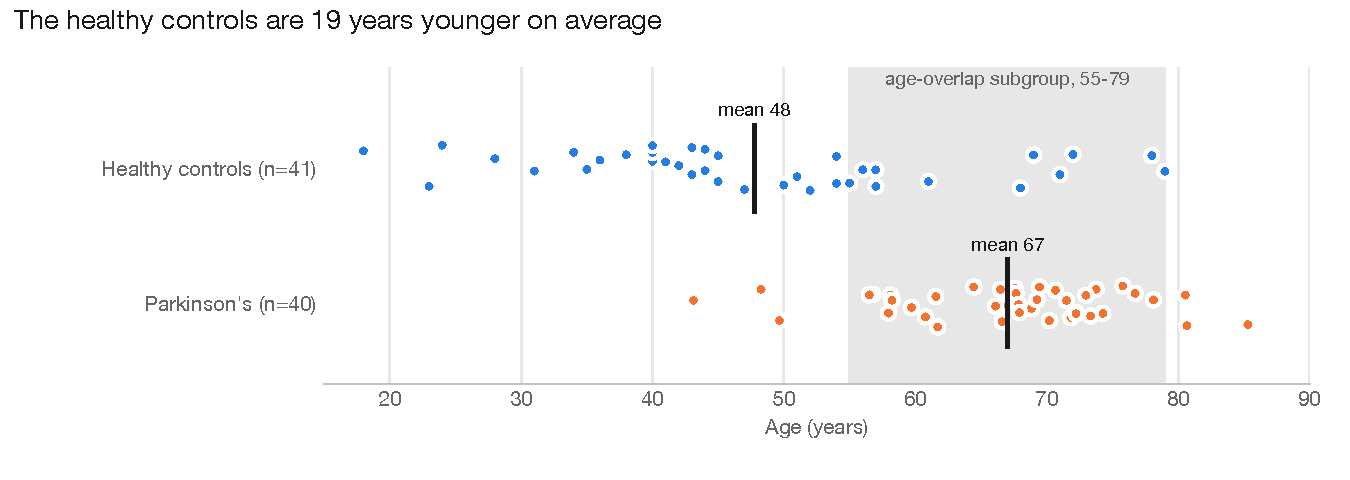
\includegraphics[width=\textwidth]{figures/02_age_by_group.pdf}
    \caption{Age of each participant by group. Black bars mark the group means. The shaded band is the 55--79 age-overlap subgroup used in Section~\ref{sec:age}.}
    \label{fig:age}
\end{figure}

\subsection{Feature Extraction}
Ninety-one acoustic features were extracted from each recording with librosa and Praat (through parselmouth)~\cite{baken1987clinical}:

\begin{itemize}
    \item \textbf{Mel-Frequency Cepstral Coefficients (MFCCs)}: mean, standard deviation, delta and delta-delta of 13 coefficients (52 features)
    \item \textbf{Fundamental frequency (F0)}: mean, standard deviation, minimum, maximum, range, coefficient of variation, median, interquartile range, skewness and kurtosis (10 features)
    \item \textbf{Formants}: mean and standard deviation of F1--F4 (8 features)
    \item \textbf{Energy}: RMS mean, standard deviation, range, minimum and maximum, and signal energy mean and standard deviation (7 features)
    \item \textbf{Voice quality}: jitter (local, absolute, RAP, PPQ5), shimmer (local, dB, APQ3, APQ5), HNR and NHR (10 features)
    \item \textbf{Spectral}: centroid, bandwidth, roll-off and zero-crossing rate (4 features)
\end{itemize}

For the CNN, 32-band mel spectrograms (8 kHz, 2048-sample window, 512-sample hop, 64 frames, reflect padding) were computed from the raw audio.

\subsection{Models}

\subsubsection{Support Vector Machine (SVM)}
An SVM with an RBF kernel (C = 10, $\gamma$ = 0.1) was trained on five features after standardization~\cite{hastie2009elements}. These hyperparameters are carried over from the original version of this work. The code does not record how they were chosen, so they are treated as fixed.

\subsubsection{Convolutional Neural Network (CNN)}
ParkCNN is a residual CNN with squeeze-and-excitation blocks and 330,273 parameters. It takes the mel spectrogram stacked with its first and second temporal differences (3 $\times$ 32 $\times$ 64). Training used AdamW (learning rate $10^{-3}$, weight decay $10^{-4}$), binary cross-entropy, batch size 16, mixup ($\alpha$ = 0.2), gradient clipping at 1.0, ReduceLROnPlateau (patience 5, factor 0.5) and early stopping (patience 10, at most 50 epochs). Each training recording was used once clean and once with each of three waveform augmentations (additive noise, time stretch in [0.92, 1.08], pitch shift in [$-$0.5, 0.5] semitones), followed by SpecAugment masking. For speed, five variants per recording and augmentation type were generated once with a fixed seed, and one was drawn per epoch.

\subsubsection{Demographic baselines}
A logistic regression on age and sex only, with no audio, measures how much of the task can be solved without the voice. An SVM on age, sex and the five selected voice features measures whether the voice adds information beyond demographics.

\subsection{Validation Protocol}
All models were evaluated with repeated stratified 5-fold cross-validation (10 repeats, 50 train/test splits, seed 42). Every model saw the same splits. Within each split, every data-dependent choice was made on the training part only:

\begin{itemize}
    \item \textbf{Feature selection}: the five features with the highest absolute correlation with the label, computed on the training fold
    \item \textbf{Decision threshold} (where tuned): the threshold in \{0.30, 0.35, \ldots, 0.70\} maximizing Youden's J on inner 5-fold cross-validated predictions of the training fold
    \item \textbf{CNN early stopping}: a stratified 20\% validation split of the training fold
\end{itemize}

Selecting features or tuning on data that is later used for testing is known to inflate performance estimates on small samples~\cite{ambroise2002selection, varma2006bias}. To measure that effect directly, the original pipeline was also re-run as first reported: five MFCC features chosen by correlation on all 81 recordings, a threshold tuned on the same leave-one-out (LOOCV) predictions it was scored on, and a CNN early-stopped on its own test fold.

Reported values are mean $\pm$ standard deviation across the 50 test folds. The standard deviation describes fold-to-fold spread. It is not a confidence interval, because the folds share participants. Metrics are accuracy, area under the ROC curve (AUC), sensitivity, specificity and F1-score.

\section{Experimental Results}

\subsection{Effect of the Evaluation Leaks}
Re-running the original pipeline reproduces the first report exactly: 82.72\% accuracy, 86.28\% AUC and 85.00\% sensitivity on a single 5-fold split, and 74.07\% accuracy on LOOCV, with sensitivity rising to 80.00\% at a threshold of 0.45 tuned on those same predictions. Table~\ref{tab:model_comparison} and Figure~\ref{fig:auc} show how these numbers change.

Repeating the same leaky SVM pipeline over 50 splits lowers accuracy to 77.1\%, so the single split was also favorable. Choosing the five features inside each training fold lowers accuracy further to 71.6\% and AUC to 0.78, with sensitivity at 68.0\%. Tuning the threshold inside each training fold does not help (69.9\% accuracy, 68.2\% sensitivity). The chosen threshold varied between 0.30 and 0.70 across folds.

The CNN scores below the SVM in both regimes. Early-stopped on its test fold, it reaches 63.0\% accuracy and 0.72 AUC. Early-stopped on a split of its training data, it reaches 60.0\% and 0.67.

\begin{table}[H]
    \centering
    \small
    \setlength{\tabcolsep}{3pt}
    \caption{Performance under repeated stratified 5-fold cross-validation (50 folds, mean $\pm$ SD). The first row is the original single 5-fold split. ``Leaky'' marks choices made with access to the test data.}
    \label{tab:model_comparison}
    \vspace{0.6em}
    \resizebox{\textwidth}{!}{%
    \begin{tabular}{lccccc}
        \hline
        \textbf{Model} & \textbf{Accuracy} & \textbf{AUC} & \textbf{Sensitivity} & \textbf{Specificity} & \textbf{F1} \\
        \hline
        SVM, as first reported (leaky, 1 split) & 82.7 $\pm$ 6.8 & 86.3 $\pm$ 5.7 & 85.0 $\pm$ 13.7 & 80.6 $\pm$ 6.4 & 82.5 $\pm$ 8.0 \\
        SVM, same pipeline (leaky) & 77.1 $\pm$ 8.1 & 83.7 $\pm$ 6.9 & 78.5 $\pm$ 15.2 & 75.6 $\pm$ 12.4 & 76.6 $\pm$ 9.6 \\
        \textbf{SVM, features chosen in-fold} & \textbf{71.6 $\pm$ 11.3} & \textbf{78.1 $\pm$ 11.3} & \textbf{68.0 $\pm$ 17.3} & \textbf{75.1 $\pm$ 15.7} & \textbf{69.7 $\pm$ 12.5} \\
        SVM, features and threshold in-fold & 69.9 $\pm$ 10.0 & 78.1 $\pm$ 11.3 & 68.2 $\pm$ 18.8 & 71.6 $\pm$ 19.7 & 68.3 $\pm$ 12.1 \\
        ParkCNN, early-stopped on test fold (leaky) & 63.0 $\pm$ 10.8 & 72.0 $\pm$ 10.4 & 58.8 $\pm$ 19.9 & 67.3 $\pm$ 22.7 & 59.8 $\pm$ 13.9 \\
        \textbf{ParkCNN, early-stopped in-fold} & \textbf{60.0 $\pm$ 9.6} & \textbf{66.6 $\pm$ 12.8} & \textbf{52.8 $\pm$ 25.3} & \textbf{67.1 $\pm$ 23.3} & \textbf{53.8 $\pm$ 17.1} \\
        \hline
        \textbf{Age + sex only (logistic regression)} & \textbf{81.8 $\pm$ 10.2} & \textbf{85.6 $\pm$ 9.0} & \textbf{80.8 $\pm$ 16.0} & \textbf{82.8 $\pm$ 10.6} & \textbf{80.8 $\pm$ 12.1} \\
        Age + sex only (SVM) & 82.0 $\pm$ 9.6 & 86.0 $\pm$ 9.4 & 85.5 $\pm$ 13.4 & 78.6 $\pm$ 12.6 & 82.2 $\pm$ 10.1 \\
        Voice (in-fold) + age + sex (SVM) & 78.6 $\pm$ 10.2 & 86.1 $\pm$ 9.5 & 79.0 $\pm$ 15.2 & 78.2 $\pm$ 13.6 & 78.1 $\pm$ 11.6 \\
        \hline
    \end{tabular}%
    }
\end{table}

\begin{figure}[H]
    \centering
    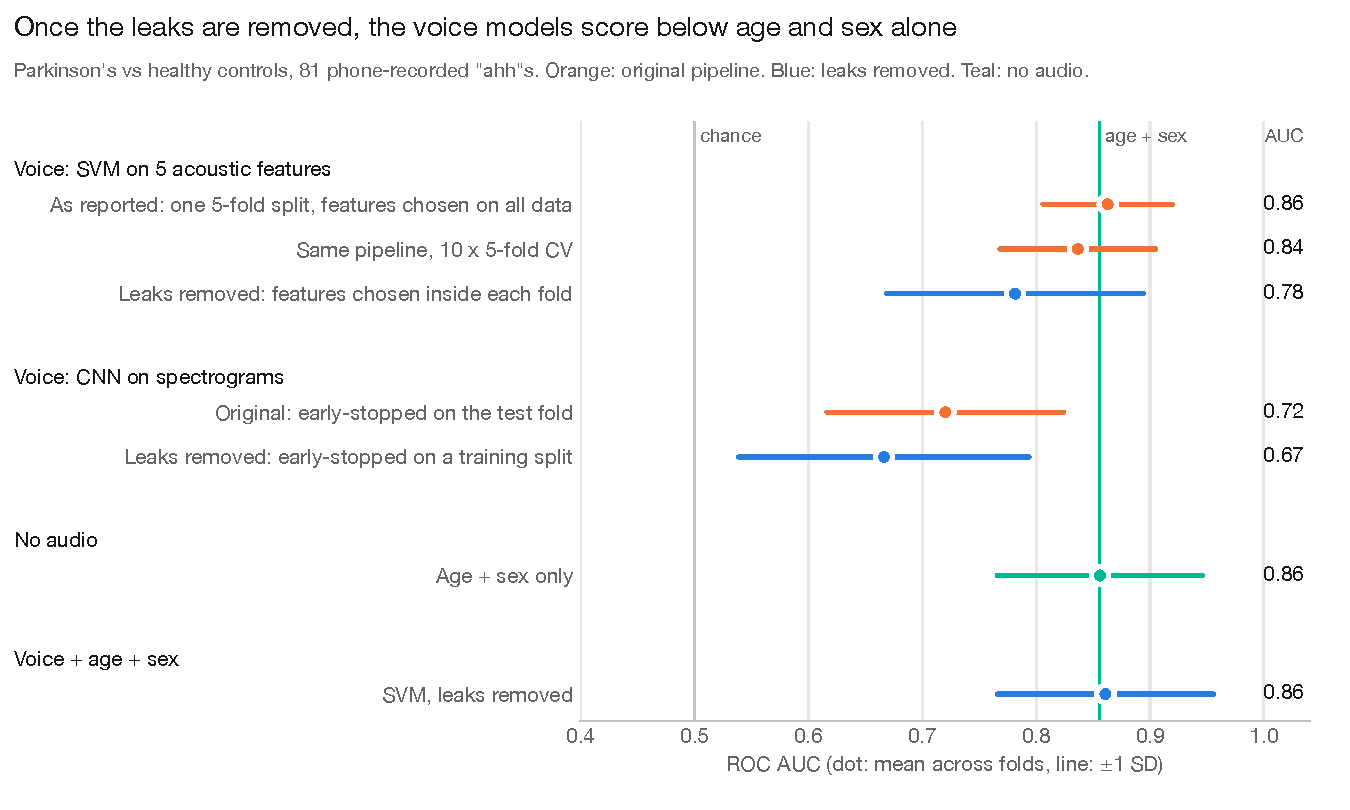
\includegraphics[width=\textwidth]{figures/01_auc_by_model.pdf}
    \caption{AUC by model (dot: mean over 50 folds; line: $\pm$1 SD). Orange: original pipeline with leaks. Blue: leaks removed. Teal: age and sex only. The teal vertical line marks the age + sex baseline.}
    \label{fig:auc}
\end{figure}

\subsection{Selected Features}
When selection happens inside each training fold, the selected set changes from fold to fold. The range of RMS energy (\texttt{rms\_range}) was selected in all 50 folds, followed by \texttt{mfcc\_std\_1} (39), \texttt{mfcc\_mean\_2} (31), \texttt{mfcc\_std\_2} (28) and \texttt{rms\_max} (23). Two of the five MFCC features of the original model, \texttt{mfcc\_std\_11} and \texttt{mfcc\_std\_12}, were selected in only 10 and 9 folds.

\subsection{The Age Confound}
\label{sec:age}
A logistic regression on age and sex alone reaches 81.8\% accuracy and 0.86 AUC, higher than every voice-only model once the leaks are removed (Table~\ref{tab:model_comparison}). Adding the five in-fold voice features to age and sex changes the AUC by $+0.001 \pm 0.089$ (same SVM, same folds), with an improvement in only 24 of 50 folds. Across the full dataset, the voice therefore adds no measurable information beyond age and sex.

To test whether any voice signal remains when age is controlled, the analysis was repeated in the subgroup aged 55--79. This range was fixed from the ages alone, before any model was scored on it. It contains 11 controls (mean age 65.7) and 34 participants with PD (mean age 67.5). With so few controls, the AUC was computed on pooled out-of-fold predictions for each of 10 repeats of 5-fold cross-validation. In this subgroup, age and sex no longer separate the groups (AUC 0.32). The in-fold voice SVM reaches an AUC of $0.66 \pm 0.09$. In a permutation test that repeated the full procedure on 1,000 label shuffles within the subgroup, the shuffled AUCs averaged 0.49 and the observed value gives $p = 0.037$ (Figure~\ref{fig:subgroup}).

\begin{figure}[H]
    \centering
    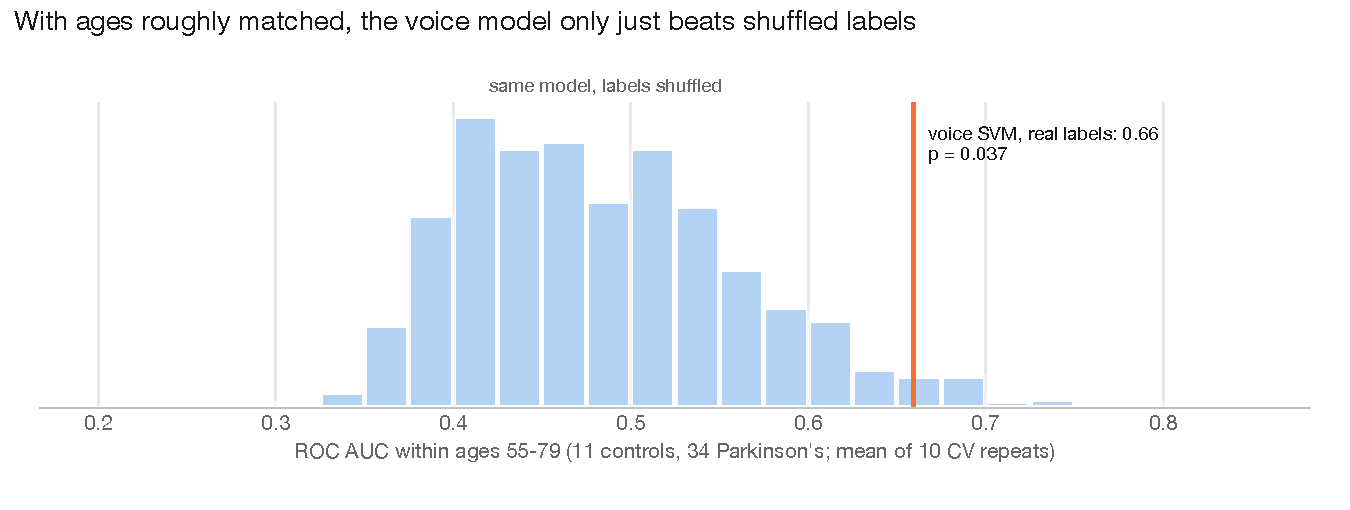
\includegraphics[width=\textwidth]{figures/03_subgroup_permutation.pdf}
    \caption{Age-overlap subgroup (55--79 years). Bars: AUC of the same procedure on 1,000 label permutations. Line: AUC with the true labels.}
    \label{fig:subgroup}
\end{figure}

\section{Discussion}

\subsection{What the Corrected Results Show}
The headline result of the first version (82.72\% accuracy, 85\% sensitivity) came from three choices that used the test data: feature selection on the full dataset, a threshold tuned on the predictions it was evaluated on, and CNN early stopping on the test fold. Removing them lowers the SVM to 71.6\% accuracy and the CNN to 60.0\%. The single favorable split accounts for about 5.6 points and in-fold feature selection for another 5.5. This matches the known behavior of selection bias on small samples~\cite{ambroise2002selection, varma2006bias}.

The larger issue is the age imbalance between groups. Age and sex alone classify the dataset better than the voice, and the voice adds nothing on top of them. The current evidence therefore cannot tell whether the voice models detect Parkinson's disease or the voice changes of age. The age-matched subgroup gives a weak indication ($p = 0.037$) that some disease-related signal exists. That result rests on 11 controls and one subgroup, and it would not survive a strict correction for multiple analyses. It should be treated as a hypothesis for a larger, age-matched sample.

\subsection{Comparison with Prior Work}
High accuracies are common in the literature (Table~\ref{tab:ml_pd}), but they are hard to compare. Datasets, recording conditions and validation protocols differ, and reports rarely state whether feature selection happened inside the cross-validation loop. The corrected results here (0.78 AUC for the SVM on 8 kHz telephone audio) are in line with the 0.6--0.7 AUC that \citet{carron2021mobile} found for uncontrolled smartphone recordings. They should not be compared directly with laboratory-quality studies.

\subsection{Traditional ML vs. Deep Learning on Small Datasets}
The SVM outperformed the CNN in both the leaky and the corrected setting (0.78 vs. 0.67 AUC corrected). With 81 recordings and a 330,273-parameter network, this ordering is expected. It is the one conclusion of the first version that holds after correction. Both models nevertheless fall below the demographic baseline, so neither can be recommended for screening on this evidence.

\subsection{Limitations}
\begin{itemize}
    \item \textbf{Age confound}: the groups differ by 19 years on average, and the age-matched subgroup is small (11 controls).
    \item \textbf{Recording conditions}: the most consistently selected feature (\texttt{rms\_range}) depends on loudness, which over the phone also depends on microphone distance and device.
    \item \textbf{Fixed SVM hyperparameters}: C = 10 and $\gamma$ = 0.1 were not tuned here, and their origin is undocumented. If they were chosen on the full dataset, a small leak remains in all SVM results.
    \item \textbf{Small, single-source data}: 81 participants, one vowel task and one dataset. There is no external validation and no information on disease stage or medication.
    \item \textbf{Variance estimates}: fold standard deviations understate uncertainty, because folds share participants.
\end{itemize}

\subsection{Future Work}
\begin{enumerate}
    \item Evaluate on age- and sex-matched cohorts, or include age as a covariate in every comparison
    \item Validate on an independent dataset recorded under different conditions
    \item Tune hyperparameters inside nested cross-validation
    \item Test connected speech and other vocal tasks in addition to the sustained vowel
\end{enumerate}

\section{Conclusion}
This study re-examined a voice-based Parkinson's disease classifier trained on 81 telephone recordings of a sustained vowel. The originally reported 82.72\% accuracy did not survive a leak-free evaluation. Under repeated stratified cross-validation, with every choice made inside the training folds, the SVM reached 71.6\% accuracy (0.78 AUC) and the CNN 60.0\% (0.67 AUC). A model using only age and sex reached 81.8\% (0.86 AUC), and adding voice features to it gave no improvement. On this dataset, voice-based detection of Parkinson's disease cannot be separated from age. A weak residual signal in an age-matched subgroup ($p = 0.037$, 11 controls) motivates testing on larger, age-matched data before any clinical claim is made.

% References
\bibliography{references}

\end{document}
